% !TEX TS-program = pdflatex
% !TEX encoding = UTF-8 Unicode

% This is a simple template for a LaTeX document using the "article" class.
% See "book", "report", "letter" for other types of document.

\documentclass[11pt]{article} % use larger type; default would be 10pt

\usepackage[utf8]{inputenc} % set input encoding (not needed with XeLaTeX)

%%% Examples of Article customizations
% These packages are optional, depending whether you want the features they provide.
% See the LaTeX Companion or other references for full information.

%%% PAGE DIMENSIONS
\usepackage{geometry} % to change the page dimensions
\geometry{a4paper} % or letterpaper (US) or a5paper or....
% \geometry{margin=2in} % for example, change the margins to 2 inches all round
% \geometry{landscape} % set up the page for landscape
%   read geometry.pdf for detailed page layout information

\usepackage{graphicx} % support the \includegraphics command and options

% \usepackage[parfill]{parskip} % Activate to begin paragraphs with an empty line rather than an indent

%%% PACKAGES
\usepackage{booktabs} % for much better looking tables
\usepackage{array} % for better arrays (eg matrices) in maths
\usepackage{paralist} % very flexible & customizable lists (eg. enumerate/itemize, etc.)
\usepackage{verbatim} % adds environment for commenting out blocks of text & for better verbatim
\usepackage{subfig} % make it possible to include more than one captioned figure/table in a single float
% These packages are all incorporated in the memoir class to one degree or another...

%%% HEADERS & FOOTERS
\usepackage{fancyhdr} % This should be set AFTER setting up the page geometry
\pagestyle{fancy} % options: empty , plain , fancy
\renewcommand{\headrulewidth}{0pt} % customise the layout...
\lhead{}\chead{}\rhead{}
\lfoot{}\cfoot{\thepage}\rfoot{}

%%% SECTION TITLE APPEARANCE
\usepackage{sectsty}
\allsectionsfont{\sffamily\mdseries\upshape} % (See the fntguide.pdf for font help)
% (This matches ConTeXt defaults)

%%% ToC (table of contents) APPEARANCE
\usepackage[nottoc,notlof,notlot]{tocbibind} % Put the bibliography in the ToC
\usepackage[titles,subfigure]{tocloft} % Alter the style of the Table of Contents
\renewcommand{\cftsecfont}{\rmfamily\mdseries\upshape}
\renewcommand{\cftsecpagefont}{\rmfamily\mdseries\upshape} % No bold!

% MATH
\usepackage{graphicx}
\usepackage{subfig}

\usepackage{mathtools}
\usepackage{amsmath}
\usepackage{float}
\usepackage{listings}
%%% END Article customizations

%%% The "real" document content comes below...

\title{Numerical Optimization - Handin 5}
\author{Martin Simon Haugaard - CDL966}
%\date{} % Activate to display a given date or no date (if empty),
         % otherwise the current date is printed 

\begin{document}
\maketitle
\section*{10.1}
It's given that: \\
$J$ is an $m~x ~n$ matrix, with $m \leq n$,\\
vector $y \in R^m$\

In order to show that $J$ has full column rank iff $J^T J$ is nonsingular, the goal is to show that
\begin{gather*}\text{"J has full column rank"}\implies\text{"$J^T J$ is nonsingular"}\\
\text{"$J^T J$ is nonsingular"}\implies\text{"J has full column rank"} \end{gather*}

A full-rank matrix is also linearly independent, so from \textit{"J has full column rank}" \begin{gather}J  x = 0 \implies x = 0\end{gather}
$J^T J$ being nonsingular means that
\begin{gather}
J^T J x= 0 \implies x = 0
\end{gather}
\subsection*{\textbf{a)}}
Now the goal is to prove that they each imply each other.
\begin{gather*}
J^T J x= 0 \implies \\
x^T J^T J x = x^T * 0 \implies x^T J^T J x = 0  \implies (x J)^T J x  = 0\implies (J x)  (J x)  = 0\implies\\ || J x|| ^2  = 0\implies\\ J x = 0 \implies x = 0
\end{gather*}
Which is what was desired. Next 
\begin{gather*}
Jx = 0 \implies J^T Jx = J^T * 0 \implies \\J^T Jx = 0 \implies x = 0
\end{gather*}
%\subsection*{\textbf{b}}
\section*{10.2}
To prove that $f(x) = \frac{1}{2} || Jx - y || ^2$ is convex, it's sufficient to prove that the second derivative is positive for all values of $x$ the interval in question, which is $R$.
\begin{gather*}
f(x) = \frac{1}{2} || Jx - y || ^2\\
f'(x) = J^2 x - Jy\\
f''(x) = J^2
\end{gather*}
Which is clearly positive for any value of $x$. Hence the function is convex.

\section*{10.3}
%\subsection*{\textbf{a}}
\subsection*{\textbf{b}}
If $\Pi = I$, $J \Pi = J = Q_1 R$. Using this $J$ on the form of 10.15 gives
\begin{gather*}J^T J = (Q_ 1 R)^T (Q_1 R) = R^T R\end{gather*}A Cholesky factorization is suppose to be unique if the upper triangular has positive diagonal elements, which is the case for both $R$ and $\hat{R}$. Hence for this to be the case here $R = \hat{R}$
\section*{Programming}


%\begin{figure}[H]
%    \centering
%    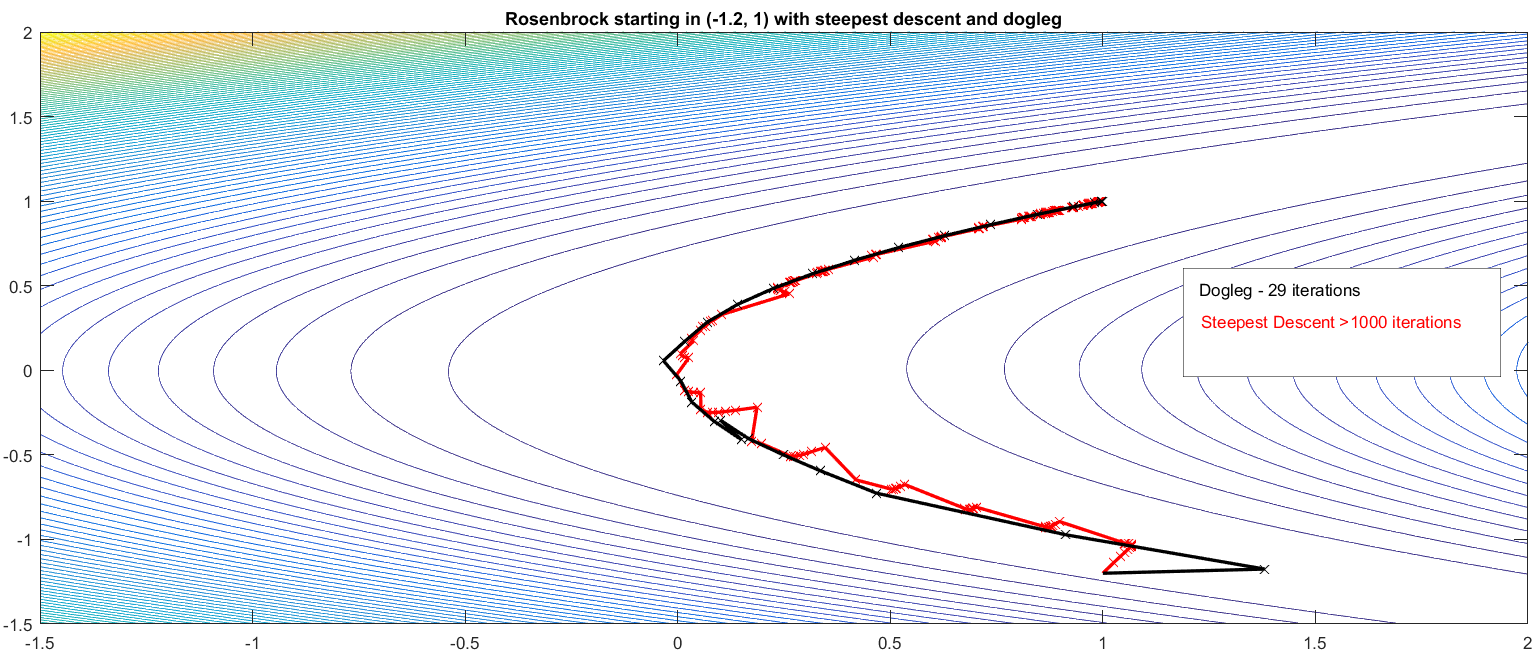
\includegraphics[width=1\textwidth]{-12_1_mixed}
%    \caption{Steepest Descent and Dogleg method, starting at $(-1.2, 1)$}
%    \label{fig:dogleg2}
%\end{figure}

\end{document}
